\documentclass[11pt,a4paper]{article}
\usepackage[utf8]{inputenc}
\usepackage[T1]{fontenc}
\usepackage{lmodern}
\usepackage{amsmath,amssymb}
\usepackage{booktabs}
\usepackage{threeparttable}
\usepackage{graphicx}
\usepackage[margin=2.6cm]{geometry}
\usepackage[font=small,labelfont=bf,labelsep=colon]{caption}
\usepackage{setspace}
\usepackage[hidelinks]{hyperref}
\usepackage{xcolor}
\usepackage{enumitem}
\usepackage[round]{natbib}

\renewcommand{\contentsname}{Indholdsfortegnelse}
\renewcommand{\figurename}{Figur}
\renewcommand{\tablename}{Tabel}
\renewcommand{\refname}{Litteratur}
\setstretch{1.08}
\setlength{\parindent}{0pt}
\setlength{\emergencystretch}{2em}
\setlength{\parskip}{0.55em}
\newcommand{\eks}{\textbf{eksplorativ}}

\begin{document}

% ---------------------------------------------------------------- forside
\begin{titlepage}
\centering
\vspace*{2.2cm}
{\large\bfseries KØBENHAVNS UNIVERSITET\par}
\vspace{0.3cm}
{\normalsize DET SAMFUNDSFAGLIGE FAKULTET\par}
{\normalsize Økonomisk Institut\par}
\vspace{3.2cm}
{\LARGE\bfseries Dollarfølsomheden i emerging markets-obligationer i lokalvaluta: lande, euroinvestorer og forudsigelighed\par}
\vspace{2.2cm}
{\large Albert Claes Poulsen\par}
\vspace{0.4cm}
{BSc Økonomi, 2. år, Københavns Universitet\par}
{gbl255@alumni.ku.dk\par}
\vspace{1.4cm}
{Selvstændigt analyseprojekt, version 2\par}
{17. november 2026\par}
\vfill
{\small Data til og med 17.11.2026 (sidste måned er ufuldstændig). Kode: \texttt{https://github.com/ACP-dev1/dollar-em}\par}
\small Version 1 (23. oktober 2026) analyserede EMLC-fonden som helhed for en dollarinvestor.\par
\end{titlepage}

\tableofcontents
\newpage

% ---------------------------------------------------------------- introduktion
\section*{Introduktion}
\addcontentsline{toc}{section}{Introduktion}

Version 1 af dette projekt viste, at en position i EM-obligationer i lokalvaluta i praksis også er en position på en svagere dollar: når Feds brede dollarindeks steg 1\,\%, faldt EMLC-fonden i gennemsnit 1,70\,\% målt i dollar. Analysen havde tre begrænsninger. Den så kun på fonden som helhed, den kunne kun opdele følsomheden i valuta og rente ved hjælp af en valutaproxy, der ikke matchede fondens lande, og den antog en investor, der måler sit afkast i dollar. For en dansk eller europæisk investor er det sidste ikke uskyldigt, fordi euroen selv bevæger sig kraftigt over for dollaren.

Denne version undersøger derfor følgende:
\emph{Hvor dollarfølsomme er emerging markets-obligationer i lokalvaluta i de enkelte lande, hvordan afhænger følsomheden af, om investoren måler sit afkast i dollar eller euro og om valutaen afdækkes, og kan afkastet forudsiges?}

Analysen bygger på månedlige afkast fra 2006 til 2026, som er konstrueret fra bunden for 12 lande ud fra spotkurser, 10-årige statsrenter og styringsrenter. Konstruktionen gør opdelingen i en valutadel og en obligationsdel eksakt, og den gør det muligt at beregne afkastet for fire investortyper: en dollarinvestor, en uafdækket euroinvestor, en euroinvestor i en dollarafdækket andelsklasse og en fuldt afdækket euroinvestor. Landene vægtes med EMLC-fondens faktiske valutavægte, som er indsamlet fra fondens indberetninger til SEC for 2010--2026. Det konstruerede aggregat har en korrelation på 0,96 med EMLC.

Analysen viser fire ting. \emph{For det første} er dollarfølsomheden meget forskellig på tværs af lande, fra $-2{,}0$ i Ungarn og $-1{,}9$ i Brasilien til $-0{,}1$ i Kina, og valutaen står for omkring tre fjerdedele af den. \emph{For det andet} er dollarfølsomheden næsten væk for en uafdækket euroinvestor: dollarbetaen falder fra $-1{,}33$ til $-0{,}19$ og er ikke signifikant på 5\,\%-niveau. Det skyldes, at euroen selv svækkes, når dollaren styrkes. Til gengæld har en euroinvestor i en andelsklasse, der afdækker dollar til euro, præcis den samme dollarrisiko som en dollarinvestor. Overraskende nok er det de centraleuropæiske lande, ikke de asiatiske, der giver euroinvestoren dollarrisiko. \emph{For det tredje} kan afkastet på EM-markedet som helhed ikke forudsiges en måned frem bedre end med det historiske gennemsnit, hverken for en dollar- eller en euroinvestor. \emph{For det fjerde} er der derimod evidens for forudsigelighed \emph{på tværs af lande}. En investor, der hver måned holdt de fire lande i EMLC-porteføljen med det stærkeste kombinerede signal (carry, momentum og value), har fået 7,5\,\% om året, mod 4,3\,\% ved blot at holde EMLC-porteføljen. Merafkastet på 3,3 procentpoint er signifikant ($t=2{,}39$), mens carry alene giver 2,4 procentpoint og ikke er signifikant på 5\,\%-niveau. For euroinvestoren har en simpel afdækningsregel hævet Sharpe-ratioen til 0,41, mod 0,36 ved altid at være uafdækket og 0,35 ved altid at være afdækket. Der er set bort fra handelsomkostninger, og forskellen i Sharpe-ratio er ikke testet statistisk.

% ---------------------------------------------------------------- teori
\section{Teoretisk ramme}

\subsection{Valutakanalen og rentekanalen}
Som i version 1 kan afkastet målt i dollar på en obligation i lokalvaluta i land $c$ tilnærmelsesvis skrives som
\begin{equation}
r^{USD}_{c,t} \;\approx\; \underbrace{y_{c,t-1} - D\,\Delta y_{c,t}}_{r^{LC}_{c,t}:\ \text{obligationsdel}} \;+\; \underbrace{\Delta e_{c,t}}_{\text{valutadel}},
\label{eq:dekomp}
\end{equation}
hvor $y$ er den lokale rente, $D$ varigheden og $\Delta e$ ændringen i værdien af den lokale valuta målt i dollar. Dollaren påvirker afkastet gennem to kanaler. \emph{Valutakanalen} er mekanisk: når dollaren styrkes, falder værdien af lokalvalutaen. \emph{Rentekanalen} virker gennem de finansielle forhold: en stærkere dollar strammer forholdene i EM og hæver risikopræmien på obligationer i lokalvaluta, fordi låntagere og udenlandske investorer har dollareksponering \citep{hofmann2020,avdjiev2019}. Dollaren er desuden en systematisk risikofaktor, der forklarer en stor del af bilaterale valutakursbevægelser \citep{verdelhan2018}.

\subsection{Euroinvestoren}
En investor, der måler sit afkast i euro, får dollarafkastet omregnet til euro:
\begin{equation}
r^{EUR}_{c,t} = r^{USD}_{c,t} - \Delta \ln \text{EURUSD}_t,
\label{eq:eur}
\end{equation}
hvor EURUSD er antal dollar pr.\ euro. Dollarbetaen for en euroinvestor er derfor
\begin{equation}
\beta^{EUR}_c = \beta^{USD}_c - \beta^{EURUSD},
\label{eq:betaeur}
\end{equation}
hvor $\beta^{EURUSD}$ er euroens egen dollarbeta. Når dollaren styrkes, falder både EM-valutaerne og euroen. Hvis de falder lige meget, har en euroinvestor ingen dollarrisiko, og eksponeringen er en ren position på EM-valutaerne mod euroen.

Valutaafdækning foretages i praksis med terminsforretninger, og afkastet af en afdækning svarer ved dækket renteparitet til renteforskellen. Det giver fire investortyper:
\begin{align}
\text{A: USD, uafdækket:}\quad & r^{A}_{c,t} = r^{LC}_{c,t} + \Delta e^{USD}_{c,t} \label{eq:A}\\
\text{B: EUR, uafdækket:}\quad & r^{B}_{c,t} = r^{LC}_{c,t} + \Delta e^{EUR}_{c,t} \label{eq:B}\\
\text{C: EUR, USD-hedged andelsklasse:}\quad & r^{C}_{c,t} = r^{A}_{c,t} + (i^{EA}_{t-1} - i^{US}_{t-1})/12 \label{eq:C}\\
\text{D: EUR, fuldt afdækket:}\quad & r^{D}_{c,t} = r^{LC}_{c,t} + (i^{EA}_{t-1} - i^{c}_{t-1})/12 \label{eq:D}
\end{align}
Type C er relevant, fordi mange europæiske EM-fonde tilbyder en ``EUR-hedged'' andelsklasse, der afdækker fondens dollarværdi til euro, men ikke de underliggende EM-valutaer. Da renteforskellen i \eqref{eq:C} er kendt på forhånd og næsten konstant fra måned til måned, har type C samme dollarbeta som type A. Type D har kun obligationsdelens dollarbeta.

Rammen giver fire forudsigelser. Obligationer i lokalvaluta bør have en negativ dollarbeta for en dollarinvestor. Valutaen bør stå for størstedelen af den. Dollarbetaen bør være numerisk mindre for en uafdækket euroinvestor. En euroinvestor i en dollarafdækket andelsklasse bør have samme dollarrisiko som en dollarinvestor.

\subsection{Forudsigelighed}
Hvis afkastet indeholder en tidsvarierende risikopræmie, kan variable, der måler præmien, forudsige det. Litteraturen om valutaafkast peger på tre: \emph{carry} (lande med høj rente har højere forventede valutaafkast, \citealp{lustig2007,lustig2011}), \emph{momentum} (valutaer, der har styrket sig, fortsætter, \citealp{menkhoff2012}) og \emph{value} (reelt billige valutaer styrkes over tid, \citealp{asness2013}). Hertil kommer global risikovillighed målt ved VIX og dollarens egen momentum. Den empiriske litteratur om aktier viser dog, at sådanne variable ofte forudsiger godt i stikprøven, men dårligt uden for den \citep{welch2008}. Forudsigelserne vurderes derfor udelukkende uden for stikprøven.

% ---------------------------------------------------------------- data og metode
\section{Data og metode}

\subsection{Data}
Analysen bygger på månedlige data fra februar 2006 til november 2026 ($N=250$ for aggregatet). Startpunktet er bestemt af Feds dollarindeks mod avancerede økonomier. Alle serier måles ved udgangen af måneden, og afkast er log-afkast i procent.

\begin{itemize}[leftmargin=1.2em,itemsep=0.15em]
\item \textbf{Lande}: Brasilien, Colombia, Indien, Indonesien, Kina, Malaysia, Mexico, Polen, Sydafrika, Thailand, Tjekkiet og Ungarn. De udgør mellem 68 og 83\,\% af EMLC-fonden over tid.
\item \textbf{Valutakurser}: ECB's daglige referencekurser mod euro omregnet til dollar via EUR/USD; Colombia fra Yahoo Finance.
\item \textbf{Renter}: 10-årige statsrenter ved månedens udgang fra investing.com for otte lande og OECD-serier via FRED for fire (Polen, Tjekkiet, Ungarn, Sydafrika). Styringsrenter for alle lande, USA og euroområdet fra BIS.
\item \textbf{Dollar}: Feds dollarindeks mod avancerede økonomier (AFE) som hovedspecifikation og det brede indeks som robusthed.
\item \textbf{Prædiktorer}: reale effektive valutakurser (BIS), VIX (FRED).
\item \textbf{Validering}: EMLC- og EMB-fondene (Yahoo Finance, justeret for udlodninger).
\item \textbf{Vægte}: EMLC-fondens valutafordeling, opgjort fra fondens beholdningsindberetninger til SEC: 28 kvartaler fra N-PORT (2019--2026) og 23 halvår fra N-Q og N-CSR (2010--2019).
\end{itemize}

\textbf{Konstruktion af afkast.} Obligationsdelen beregnes som afkastet på en 10-årig par-obligation: obligationen købes til kurs 100 med en kupon lig renten ved månedens start og værdisættes ved månedens udgang til den nye rente. Valutadelen er log-ændringen i spotkursen. De fire investortyper beregnes som i \eqref{eq:A}--\eqref{eq:D} med styringsrenter som afdækningsrenter. Landene vægtes hver måned med EMLC-fondens senest kendte valutavægte, så der ikke bruges fremtidig information. Før juli 2010, hvor fonden ikke fandtes, bruges de første vægte.

\textbf{Validering.} Dollarafkastet på det konstruerede aggregat har en korrelation på 0,96 med EMLC-fonden i 2010--2026, en hældning på 0,89 og en tracking error på 3,3 procentpoint om året. Konstruktionen fanger altså fondens bevægelser tæt, selv om den bygger på én generisk obligation pr.\ land.

\subsection{Metode}
Dollarfølsomheden estimeres med regressionen
\begin{equation}
r^{j}_{c,t} = \alpha + \beta^{j}_{c}\,\Delta \text{USD}_t + \varepsilon_{t}, \qquad j \in \{A,B,C,D\},
\label{eq:reg}
\end{equation}
for hvert land og for det vægtede aggregat. Da obligationsdelen og valutadelen summerer til afkastet, gælder $\beta^{A}_c = \beta^{FX}_c + \beta^{LC}_c$ eksakt, og begge dele er målt direkte. Hovedspecifikationen bruger AFE-indekset, fordi Feds brede indeks selv indeholder EM-valutaer som kinesisk yuan og mexicansk peso, så en del af sammenhængen ellers er mekanisk. Standardfejl er Newey-West med tre lags.

\textbf{Prognoser.} Hver måned $t$ forudsiges næste måneds overskudsafkast for aggregatet (afkast minus den amerikanske henholdsvis europæiske styringsrente) for investortype A og B. Der bruges fem prædiktorer, alle kendt på tidspunkt $t$:
\begin{itemize}[leftmargin=1.2em,itemsep=0.1em]
\item \emph{Carry}: vægtet styringsrenteforskel mod USA (A) eller euroområdet (B), med én måneds publiceringsforsinkelse.
\item \emph{Dollar-momentum}: AFE-indeksets ændring over 12 måneder.
\item \emph{Valuta-momentum}: aggregatets valutaafkast over 12 måneder.
\item \emph{Value}: minus afvigelsen i den reale effektive valutakurs fra dens historiske gennemsnit (positiv værdi = billig valuta), med én måneds forsinkelse.
\item \emph{VIX}: niveauet ved månedens udgang.
\end{itemize}
Hovedmodellen indeholder carry, dollar-momentum og VIX. Desuden estimeres hver prædiktor alene og et gennemsnit af de fem univariate prognoser \citep{rapach2010}. Modellerne estimeres i et udvidende vindue med mindst 60 måneder. Koefficienter med forkert fortegn sættes til nul \citep{campbell2008}, og benchmark er det historiske gennemsnit. Prognoserne evalueres med
\begin{equation}
R^2_{OOS} = 1 - \frac{\sum_t (r_{t+1} - \hat r^{model}_{t+1})^2}{\sum_t (r_{t+1} - \bar r_t)^2},
\end{equation}
testet med \citet{clark2007}. Den økonomiske værdi måles som gevinsten i sikkerhedsækvivalent afkast ($\Delta$CER) for en investor med risikoaversion 3, der placerer mellem 0 og 150\,\% i EM ud fra prognosen. Evalueringen går fra februar 2012 til november 2026 ($N=178$), og perioden 2022--2026 rapporteres separat som holdout.

\textbf{Tværsnit og afdækning.} For hvert land beregnes tre signaler: carry (styringsrenteforskel mod USA), momentum (valutaafkast over de seneste 12 måneder ekskl.\ den seneste) og value. Hver måned rangeres landene efter hvert signal og efter et gennemsnit af de standardiserede signaler. En long--short-strategi køber de fire højest rangerede og sælger de fire lavest rangerede, og en aktiv strategi holder de fire højest rangerede mod et ligevægtet benchmark. Strategierne kræver ingen estimation. Endelig testes en afdækningsregel for euroinvestoren: hold valutaen uafdækket, når hovedmodellen forudsiger et positivt valutaoverskudsafkast ($r^B - r^D$), og afdæk ellers.

\subsection{Hypoteser}
Tabel \ref{tab:hyp} viser hypoteserne. H1--H4 blev formuleret, efter at foreløbige estimater af aggregatet var set, og er derfor ikke uafhængige test. H5--H8 og alle prognosespecifikationer blev fastlagt i koden, før prognoserne blev kørt første gang. Det er ikke dokumenteret med et eksternt tidsstempel.

\begin{table}[h!]
\centering
\caption{Hypoteser og resultat}
\label{tab:hyp}
\small
\begin{tabular}{p{0.6cm}p{10.2cm}p{3.3cm}}
\toprule
& Hypotese & Resultat \\
\midrule
H1 & Dollarbetaen er negativ for en dollarinvestor i alle 12 lande & 11 af 12 (ikke Kina) \\
H2 & Valutaen står for over halvdelen af dollarbetaen i alle lande & 11 af 12 (ikke Indonesien) \\
H3 & Dollarbetaen er numerisk mindre for en uafdækket euroinvestor end for en dollarinvestor & Aggregat og 10 af 12 \\
H4 & En euroinvestor i en USD-hedged andelsklasse har samme dollarbeta som en dollarinvestor & Understøttes \\
\midrule
H5 & Hovedmodellen forudsiger dollarinvestorens afkast: $R^2_{OOS}>0$ og signifikant & Understøttes ikke \\
H6 & Hovedmodellen forudsiger euroinvestorens afkast: $R^2_{OOS}>0$ og signifikant & Understøttes ikke \\
H7 & Carry-strategien på tværs af lande giver et positivt og signifikant afkast & Delvist (kun med alle lande) \\
H8 & Afdækningsreglen giver euroinvestoren en højere Sharpe-ratio end altid uafdækket & Understøttes (ikke testet formelt) \\
\bottomrule
\end{tabular}
\end{table}

% ---------------------------------------------------------------- resultater
\section{Resultater}

\subsection{Dollarfølsomhed i de enkelte lande}
Tabel \ref{tab:lande} viser dollarbetaen for en dollarinvestor i hvert land opdelt i valuta og obligation. Alle lande har en negativ dollarbeta, men størrelsen varierer meget. De mest følsomme er Ungarn ($-2{,}01$), Brasilien ($-1{,}90$) og Polen ($-1{,}73$). Når dollaren stiger 1\,\%, falder ungarske statsobligationer altså omkring 2\,\% målt i dollar. De mindst følsomme er de asiatiske lande med styrede valutaer: Indien ($-0{,}47$) og Kina ($-0{,}13$), hvor Kina ikke er signifikant. Dollaren forklarer 53--62\,\% af variationen i de centraleuropæiske lande, men kun 3\,\% i Kina. H1 understøttes for 11 af 12 lande.

\begin{table}[h!]
\centering
\begin{threeparttable}
\caption{Dollarbeta for en dollarinvestor pr.\ land, opdelt i valuta og obligation}
\label{tab:lande}
\small
\begin{tabular}{lcccccc}
\toprule
 & $\beta^{USD}$ & $\beta^{FX}$ & $\beta^{LC}$ & Valutaandel & $R^2$ & Start \\
\midrule
Ungarn & $-2{,}01^{***}$ & $-1{,}54^{***}$ & $-0{,}47^{***}$ & $76$\,\% & $0{,}53$ & 2006-02 \\
 & $(-11{,}46)$ & $(-14{,}12)$ & $(-4{,}33)$ & & & \\
Brasilien & $-1{,}90^{***}$ & $-1{,}17^{***}$ & $-0{,}69^{***}$ & $62$\,\% & $0{,}33$ & 2007-02 \\
 & $(-9{,}73)$ & $(-10{,}00)$ & $(-3{,}96)$ & & & \\
Polen & $-1{,}73^{***}$ & $-1{,}55^{***}$ & $-0{,}18^{***}$ & $90$\,\% & $0{,}62$ & 2006-02 \\
 & $(-15{,}74)$ & $(-17{,}50)$ & $(-2{,}75)$ & & & \\
Tjekkiet & $-1{,}45^{***}$ & $-1{,}33^{***}$ & $-0{,}12^{**}$ & $91$\,\% & $0{,}61$ & 2006-02 \\
 & $(-16{,}82)$ & $(-18{,}45)$ & $(-2{,}00)$ & & & \\
Sydafrika & $-1{,}41^{***}$ & $-1{,}28^{***}$ & $-0{,}12^{*}$ & $91$\,\% & $0{,}29$ & 2006-02 \\
 & $(-8{,}66)$ & $(-9{,}79)$ & $(-1{,}93)$ & & & \\
Colombia & $-1{,}37^{***}$ & $-1{,}01^{***}$ & $-0{,}38^{***}$ & $73$\,\% & $0{,}19$ & 2006-02 \\
 & $(-7{,}76)$ & $(-9{,}66)$ & $(-3{,}32)$ & & & \\
Indonesien & $-1{,}35^{***}$ & $-0{,}65^{***}$ & $-0{,}70^{***}$ & $48$\,\% & $0{,}26$ & 2006-02 \\
 & $(-4{,}61)$ & $(-5{,}48)$ & $(-3{,}78)$ & & & \\
Mexico & $-1{,}34^{***}$ & $-0{,}89^{***}$ & $-0{,}44^{***}$ & $67$\,\% & $0{,}32$ & 2006-02 \\
 & $(-10{,}59)$ & $(-9{,}47)$ & $(-5{,}56)$ & & & \\
Malaysia & $-0{,}81^{***}$ & $-0{,}70^{***}$ & $-0{,}11^{*}$ & $87$\,\% & $0{,}29$ & 2006-02 \\
 & $(-7{,}82)$ & $(-10{,}91)$ & $(-1{,}83)$ & & & \\
Thailand & $-0{,}68^{***}$ & $-0{,}56^{***}$ & $-0{,}12$ & $83$\,\% & $0{,}17$ & 2006-02 \\
 & $(-4{,}24)$ & $(-8{,}72)$ & $(-0{,}95)$ & & & \\
Indien & $-0{,}47^{***}$ & $-0{,}49^{***}$ & $0{,}03$ & $106$\,\% & $0{,}11$ & 2006-02 \\
 & $(-4{,}58)$ & $(-7{,}44)$ & $(0{,}28)$ & & & \\
Kina & $-0{,}13$ & $-0{,}22^{***}$ & $0{,}09$ & --\,\% & $0{,}03$ & 2006-02 \\
 & $(-1{,}60)$ & $(-4{,}97)$ & $(1{,}49)$ & & & \\
\midrule
Vægtet aggregat & $-1{,}33^{***}$ & $-1{,}01^{***}$ & $-0{,}32^{***}$ & $76$\,\% & $0{,}53$ & 2006-02 \\
 & $(-12{,}34)$ & $(-16{,}31)$ & $(-4{,}72)$ & & & \\
\bottomrule
\end{tabular}

\begin{tablenotes}\footnotesize
\item \emph{Note:} Estimation af \eqref{eq:reg} for type A. $\beta^{FX}$ og $\beta^{LC}$ er betaerne for valutadelen og obligationsdelen og summerer til $\beta^{USD}$. Valutaandel $=\beta^{FX}/\beta^{USD}$ (udeladt for Kina, hvor $\beta^{USD}$ er tæt på nul). Dollar: Feds AFE-indeks. Newey-West $t$-værdier (3 lags) i parentes. $^{*}$, $^{**}$, $^{***}$: signifikant på 10, 5 og 1\,\%. Landene er sorteret efter dollarbeta.
\end{tablenotes}
\end{threeparttable}
\end{table}

\subsection{Valuta eller rente?}
I version 1 kunne restposten ikke tolkes entydigt som en rentekanal, fordi valutaproxyen ikke matchede fondens lande. Her er opdelingen eksakt. For aggregatet er valutabetaen $-1{,}01$ og obligationsbetaen $-0{,}32$, og valutaen står dermed for 76\,\% af dollarfølsomheden. Det ligger tæt på estimatet fra version 1 (67--74\,\%), og H2 understøttes for 11 af 12 lande. Undtagelsen er Indonesien, hvor obligationsdelen er lige så dollarfølsom som valutaen ($-0{,}70$ mod $-0{,}65$).

Obligationsbetaen er negativ og signifikant på mindst 10\,\%-niveau i ni lande og størst i Indonesien, Brasilien ($-0{,}69$), Ungarn ($-0{,}47$) og Mexico ($-0{,}44$). Flere af disse lande, især Indonesien og Mexico, har i store dele af perioden haft mange udenlandske investorer i statsgælden, hvilket er konsistent med rentekanalen hos \citet{hofmann2020}: når dollaren styrkes, sælger udenlandske investorer, og de lokale renter stiger. I Kina og Indien, hvor udenlandske investorer længe har haft begrænset adgang, er obligationsbetaen nul.

\subsection{Euro- eller dollarinvestor?}
Tabel \ref{tab:agg} viser dollarbetaen for de fire investortyper. For en dollarinvestor er betaen $-1{,}33$ ($t=-12{,}3$), og dollaren forklarer 53\,\% af variationen. For en uafdækket euroinvestor er betaen kun $-0{,}19$ ($t=-1{,}9$), og dollaren forklarer 2\,\%. Forskellen følger direkte af \eqref{eq:betaeur}: euroens egen dollarbeta er $-1{,}14$, så $-1{,}33 - (-1{,}14) = -0{,}19$. Når dollaren styrkes, falder euroen næsten lige så meget som EM-valutaerne, og for euroinvestoren udligner de to bevægelser hinanden. H3 understøttes.

\begin{table}[h!]
\centering
\begin{threeparttable}
\caption{Dollarbeta for fire investortyper, vægtet aggregat og EMLC}
\label{tab:agg}
\small
\begin{tabular}{lcccc}
\toprule
 & \multicolumn{2}{c}{AFE-indeks (uden EM)} & \multicolumn{2}{c}{Bredt indeks (inkl. EM)} \\
\cmidrule(lr){2-3}\cmidrule(lr){4-5}
Investor & $\beta$ & $R^2$ & $\beta$ & $R^2$ \\
\midrule
A: USD, uafdækket & $-1{,}33^{***}$ & $0{,}53$ & $-1{,}82^{***}$ & $0{,}70$ \\
 & $(-12{,}34)$ & & $(-18{,}19)$ & \\
B: EUR, uafdækket & $-0{,}19^{*}$ & $0{,}02$ & $-0{,}54^{***}$ & $0{,}11$ \\
 & $(-1{,}90)$ & & $(-4{,}27)$ & \\
C: EUR, USD-hedged andelsklasse & $-1{,}33^{***}$ & $0{,}53$ & $-1{,}82^{***}$ & $0{,}70$ \\
 & $(-12{,}41)$ & & $(-18{,}29)$ & \\
D: EUR, fuldt afdækket & $-0{,}32^{***}$ & $0{,}16$ & $-0{,}45^{***}$ & $0{,}22$ \\
 & $(-4{,}76)$ & & $(-6{,}53)$ & \\
\midrule
EMLC-ETF, USD-investor & $-1{,}26^{***}$ & $0{,}55$ & $-1{,}70^{***}$ & $0{,}74$ \\
 & $(-13{,}13)$ & & $(-19{,}34)$ & \\
EMLC-ETF, EUR-investor & $-0{,}15$ & $0{,}01$ & $-0{,}50^{***}$ & $0{,}11$ \\
 & $(-1{,}28)$ & & $(-3{,}42)$ & \\
\bottomrule
\end{tabular}

\begin{tablenotes}\footnotesize
\item \emph{Note:} Aggregatet er vægtet med EMLC-fondens historiske valutavægte, 2006--2026 ($N=250$). EMLC-ETF: fondens udlodningsjusterede afkast, 2010--2026 ($N=196$); for euroinvestoren omregnet med \eqref{eq:eur}. Newey-West $t$-værdier i parentes.
\end{tablenotes}
\end{threeparttable}
\end{table}

Euroinvestoren i en dollarafdækket andelsklasse (type C) har en dollarbeta på $-1{,}33$, præcis som dollarinvestoren. H4 understøttes. Det er en vigtig praktisk pointe: en andelsklasse, der omtales som ``afdækket'', fjerner euroinvestorens risiko på dollaren mod euroen, men den bringer dollarrisikoen fra EM-valutaerne tilbage. Afdækningen fjerner med andre ord den forkerte risiko. Den fuldt afdækkede euroinvestor (type D) har kun obligationsdelens dollarbeta på $-0{,}32$.

Resultatet bekræftes på selve EMLC-fonden. Med AFE-indekset er dollarbetaen $-1{,}26$ for en dollarinvestor og $-0{,}15$ ($t=-1{,}3$) for en euroinvestor. Med det brede dollarindeks bliver alle betaer større, fordi indekset selv indeholder EM-valutaer. Her har euroinvestoren en signifikant beta på $-0{,}54$. Den er dog stadig kun en tredjedel af dollarinvestorens.

Billedet på landeniveau er mere nuanceret (tabel \ref{tab:invlande} og figur \ref{fig:lande}). Forventningen var, at de centraleuropæiske valutaer, som følger euroen tæt, ville have en dollarbeta tæt på nul for en euroinvestor. Det er ikke tilfældet. Ungarn ($-0{,}87$), Brasilien ($-0{,}77$), Polen ($-0{,}59$) og Tjekkiet ($-0{,}31$) har alle negative og signifikante betaer for euroinvestoren. Forklaringen er, at disse valutaer svækkes \emph{mere} end euroen, når dollaren styrkes. Det er typisk i perioder med global uro, hvor risikovilligheden falder. Omvendt har de asiatiske lande med styrede valutaer, Kina ($+1{,}01$), Indien ($+0{,}68$), Thailand og Malaysia, \emph{positive} betaer for euroinvestoren. Deres valutaer følger dollaren, så for en euroinvestor fungerer de som en dollarposition. Kina og Indien er de to lande, hvor H3 ikke holder. På aggregeret niveau udligner de to grupper hinanden.

\begin{table}[h!]
\centering
\begin{threeparttable}
\caption{Dollarbeta pr.\ land for fire investortyper}
\label{tab:invlande}
\small
\begin{tabular}{lcccc}
\toprule
 & A: USD, uafd. & B: EUR, uafd. & C: EUR, USD-hedged & D: EUR, fuldt afd. \\
\midrule
Ungarn & $-2{,}01^{***}$ & $-0{,}87^{***}$ & $-2{,}01^{***}$ & $-0{,}47^{***}$ \\
 & $(-11{,}46)$ & $(-5{,}73)$ & $(-11{,}51)$ & $(-4{,}31)$ \\
Brasilien & $-1{,}90^{***}$ & $-0{,}77^{***}$ & $-1{,}89^{***}$ & $-0{,}70^{***}$ \\
 & $(-9{,}73)$ & $(-3{,}91)$ & $(-9{,}76)$ & $(-4{,}04)$ \\
Polen & $-1{,}73^{***}$ & $-0{,}59^{***}$ & $-1{,}73^{***}$ & $-0{,}18^{***}$ \\
 & $(-15{,}74)$ & $(-6{,}75)$ & $(-15{,}90)$ & $(-2{,}82)$ \\
Tjekkiet & $-1{,}45^{***}$ & $-0{,}31^{***}$ & $-1{,}45^{***}$ & $-0{,}13^{**}$ \\
 & $(-16{,}82)$ & $(-3{,}95)$ & $(-16{,}65)$ & $(-2{,}01)$ \\
Sydafrika & $-1{,}41^{***}$ & $-0{,}27^{*}$ & $-1{,}40^{***}$ & $-0{,}13^{*}$ \\
 & $(-8{,}66)$ & $(-1{,}71)$ & $(-8{,}67)$ & $(-1{,}94)$ \\
Colombia & $-1{,}37^{***}$ & $-0{,}27$ & $-1{,}37^{***}$ & $-0{,}38^{***}$ \\
 & $(-7{,}76)$ & $(-1{,}33)$ & $(-7{,}69)$ & $(-3{,}32)$ \\
Indonesien & $-1{,}35^{***}$ & $-0{,}21$ & $-1{,}35^{***}$ & $-0{,}70^{***}$ \\
 & $(-4{,}61)$ & $(-0{,}75)$ & $(-4{,}62)$ & $(-3{,}80)$ \\
Mexico & $-1{,}34^{***}$ & $-0{,}19$ & $-1{,}33^{***}$ & $-0{,}44^{***}$ \\
 & $(-10{,}59)$ & $(-1{,}52)$ & $(-10{,}60)$ & $(-5{,}47)$ \\
Malaysia & $-0{,}81^{***}$ & $0{,}33^{***}$ & $-0{,}81^{***}$ & $-0{,}11^{*}$ \\
 & $(-7{,}82)$ & $(2{,}82)$ & $(-7{,}75)$ & $(-1{,}85)$ \\
Thailand & $-0{,}68^{***}$ & $0{,}46^{***}$ & $-0{,}68^{***}$ & $-0{,}12$ \\
 & $(-4{,}24)$ & $(2{,}85)$ & $(-4{,}21)$ & $(-0{,}96)$ \\
Indien & $-0{,}47^{***}$ & $0{,}68^{***}$ & $-0{,}46^{***}$ & $0{,}02$ \\
 & $(-4{,}58)$ & $(6{,}33)$ & $(-4{,}50)$ & $(0{,}18)$ \\
Kina & $-0{,}13$ & $1{,}01^{***}$ & $-0{,}13$ & $0{,}09$ \\
 & $(-1{,}60)$ & $(8{,}83)$ & $(-1{,}51)$ & $(1{,}41)$ \\
\midrule
Vægtet aggregat & $-1{,}33^{***}$ & $-0{,}19^{*}$ & $-1{,}33^{***}$ & $-0{,}32^{***}$ \\
 & $(-12{,}34)$ & $(-1{,}90)$ & $(-12{,}41)$ & $(-4{,}76)$ \\
\bottomrule
\end{tabular}

\begin{tablenotes}\footnotesize
\item \emph{Note:} Estimation af \eqref{eq:reg} for hver investortype, jf.\ \eqref{eq:A}--\eqref{eq:D}. AFE-dollarindeks. Newey-West $t$-værdier i parentes.
\end{tablenotes}
\end{threeparttable}
\end{table}

\begin{figure}[h!]
\centering
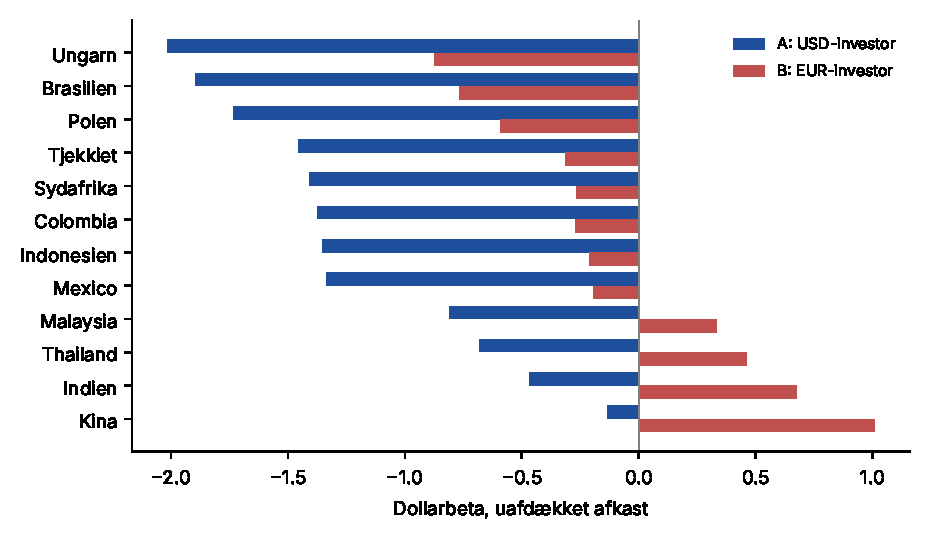
\includegraphics[width=0.86\textwidth]{resultater/fig_lande.pdf}
\caption{Dollarbeta pr.\ land for en uafdækket dollar- og euroinvestor}
\label{fig:lande}
\end{figure}

Figur \ref{fig:rullende} viser, at forskellen mellem de to investorer har været stabil over tid. Dollarinvestorens rullende beta har ligget mellem $-2{,}2$ og $-0{,}9$ og er senest $-1{,}0$. Euroinvestorens har svinget omkring nul, mellem $-1{,}0$ og $+0{,}3$, og er senest nul. Den uafdækkede euroinvestor har desuden haft en lavere volatilitet end dollarinvestoren (9,9 mod 13,0\,\% om året) og et lidt højere gennemsnitligt afkast (4,7 mod 4,2\,\% om året) i perioden.

\begin{figure}[h!]
\centering
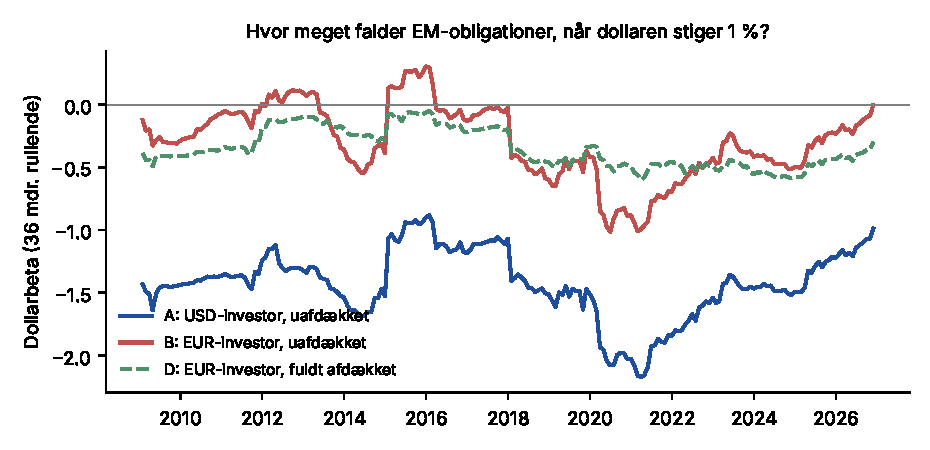
\includegraphics[width=0.86\textwidth]{resultater/fig_rullende.pdf}
\caption{Rullende dollarbeta (36 måneder) for det vægtede aggregat}
\label{fig:rullende}
\end{figure}

\subsection{Robusthed}
Tabel \ref{tab:rob} viser, at hovedresultatet er stabilt. Dollarinvestorens beta er $-1{,}34$ i 2006--2014 og $-1{,}32$ i 2015--2026, og euroinvestorens er ikke signifikant på 5\,\%-niveau i nogen af dem. Resultaterne afhænger heller ikke af 2020.

Asymmetrien fra version 1 genfindes i punktestimaterne: dollarinvestorens beta er $-1{,}48$ i måneder med stigende dollar og $-1{,}16$ i måneder med faldende. Forskellen er dog ikke signifikant ($p=0{,}22$), som i version 1.

Når der kontrolleres for ændringer i VIX, den amerikanske 10-årige rente og olieprisen, falder dollarinvestorens beta til $-1{,}06$, og euroinvestorens bliver $+0{,}11$ og insignifikant. Både VIX og den amerikanske rente har signifikante og næsten ens effekter for de to investorer: en stigning i den amerikanske rente på 1 procentpoint er forbundet med et fald på omkring 2,5--2,8\,\%. Euroinvestoren slipper altså for dollarrisikoen, men ikke for den globale risikovillighed og de amerikanske renter.

\begin{table}[h!]
\centering
\begin{threeparttable}
\caption{Robusthed: delperioder, asymmetri og kontroller}
\label{tab:rob}
\small
\begin{tabular}{lcccc}
\toprule
 & \multicolumn{2}{c}{A: USD, uafdækket} & \multicolumn{2}{c}{B: EUR, uafdækket} \\
\cmidrule(lr){2-3}\cmidrule(lr){4-5}
 & $\beta$ & $t$ & $\beta$ & $t$ \\
\midrule
Hele perioden & $-1{,}33^{***}$ & $(-12{,}34)$ & $-0{,}19^{*}$ & $(-1{,}90)$ \\
2006--2014 & $-1{,}34^{***}$ & $(-7{,}96)$ & $-0{,}12$ & $(-0{,}90)$ \\
2015--2026 & $-1{,}32^{***}$ & $(-9{,}97)$ & $-0{,}26^{*}$ & $(-1{,}67)$ \\
Uden 2020 & $-1{,}30^{***}$ & $(-11{,}89)$ & $-0{,}16$ & $(-1{,}64)$ \\
\midrule
$\beta^{op}$ (stigende dollar) & $-1{,}48^{***}$ & $(-8{,}70)$ & $-0{,}23$ & $(-1{,}26)$ \\
$\beta^{ned}$ (faldende dollar) & $-1{,}16^{***}$ & $(-7{,}07)$ & $-0{,}15$ & $(-0{,}91)$ \\
$p$-værdi, $\beta^{op}=\beta^{ned}$ & $0{,}22$ & & $0{,}76$ & \\
\midrule
$\Delta$USD, med kontroller & $-1{,}06^{***}$ & $(-10{,}69)$ & $0{,}11$ & $(1{,}06)$ \\
$\Delta$VIX & $-0{,}17^{***}$ & $(-5{,}32)$ & $-0{,}18^{***}$ & $(-5{,}51)$ \\
$\Delta y^{US}_{10}$ & $-2{,}51^{***}$ & $(-3{,}38)$ & $-2{,}78^{***}$ & $(-3{,}14)$ \\
$\Delta$Olie & $0{,}02$ & $(0{,}81)$ & $0{,}04$ & $(1{,}22)$ \\
\bottomrule
\end{tabular}

\begin{tablenotes}\footnotesize
\item \emph{Note:} Vægtet aggregat, AFE-dollarindeks. Asymmetri: \eqref{eq:reg} med separate betaer for $\max(\Delta\text{USD},0)$ og $\min(\Delta\text{USD},0)$, Wald-test. Kontroller: ændring i VIX (point), den amerikanske 10-årige rente (procentpoint) og Brent-olie (log-\%). Newey-West $t$-værdier i parentes.
\end{tablenotes}
\end{threeparttable}
\end{table}

% ---------------------------------------------------------------- prognoser
\section{Kan afkastet forudsiges?}

\subsection{Markedet som helhed}
Tabel \ref{tab:prog} viser, at ingen af modellerne forudsiger næste måneds afkast bedre end det historiske gennemsnit. Alle $R^2_{OOS}$ er negative eller nul for både dollar- og euroinvestoren, og ingen er signifikante på 5\,\%-niveau. Hitraterne på 56--60\,\% er ikke højere end andelen af måneder med positivt overskudsafkast (59\,\% for dollarinvestoren og 61\,\% for euroinvestoren), som en model, der altid forudsiger et positivt afkast, ville ramme. H5 og H6 understøttes ikke.

\begin{table}[h!]
\centering
\begin{threeparttable}
\caption{Forudsigelse af næste måneds overskudsafkast uden for stikprøven}
\label{tab:prog}
\footnotesize
\setlength{\tabcolsep}{4pt}
\begin{tabular}{lrrrrrrrr}
\toprule
 & \multicolumn{4}{c}{A: USD-investor} & \multicolumn{4}{c}{B: EUR-investor} \\
\cmidrule(lr){2-5}\cmidrule(lr){6-9}
Model & $R^2_{OOS}$ & CW $p$ & Hit & $\Delta$CER & $R^2_{OOS}$ & CW $p$ & Hit & $\Delta$CER \\
\midrule
Carry & $-0{,}19$ & $0{,}92$ & $60$ & $-0{,}52$ & $-0{,}48$ & $0{,}67$ & $59$ & $-0{,}14$ \\
Dollar-momentum & $-0{,}02$ & $0{,}90$ & $59$ & $-0{,}04$ & $-0{,}02$ & $0{,}39$ & $60$ & $0{,}51$ \\
Valuta-momentum & $-0{,}12$ & $0{,}84$ & $61$ & $-0{,}12$ & $-0{,}33$ & $0{,}88$ & $61$ & $-0{,}15$ \\
Value (REER) & $-4{,}63$ & $0{,}77$ & $57$ & $-0{,}71$ & $-3{,}29$ & $0{,}71$ & $60$ & $0{,}72$ \\
VIX & $-0{,}31$ & $0{,}57$ & $60$ & $0{,}25$ & $-0{,}49$ & $0{,}82$ & $60$ & $-0{,}06$ \\
\midrule
Hovedmodel (carry, dollar-mom., VIX) & $-1{,}31$ & $0{,}53$ & $56$ & $0{,}87$ & $-2{,}67$ & $0{,}12$ & $57$ & $2{,}54$ \\
Kombination (gns. af univariate) & $-0{,}63$ & $0{,}90$ & $59$ & $-1{,}21$ & $-0{,}83$ & $0{,}91$ & $60$ & $-0{,}05$ \\
\bottomrule
\end{tabular}

\begin{tablenotes}\footnotesize
\item \emph{Note:} Vægtet aggregat, februar 2012 -- november 2026 ($N=178$; univariate modeller med længere data har op til 226 observationer). Udvidende vindue med mindst 60 måneder, fortegnsbegrænsede koefficienter. $R^2_{OOS}$ i procent mod det historiske gennemsnit. CW $p$: ensidet Clark-West-test. Hit: andel måneder, hvor prognosen rammer fortegnet på overskudsafkastet (\%). $\Delta$CER: gevinst i sikkerhedsækvivalent afkast i procentpoint p.a.\ for en investor med risikoaversion 3.
\end{tablenotes}
\end{threeparttable}
\end{table}

Det mest interessante resultat er hovedmodellen for euroinvestoren. Den har et negativt $R^2_{OOS}$ ($-2{,}7$\,\%), men Clark-West-testen er tæt på signifikans ($p=0{,}12$), og en investor, der havde brugt modellen, ville have opnået en gevinst på 2,5 procentpoint i sikkerhedsækvivalent afkast. Testen tager højde for, at en større model bliver straffet for estimationsstøj, og resultatet antyder, at modellen indeholder information, som ikke slår igennem i kvadratfejlen. Tabel \ref{tab:perioder} viser dog, at gevinsten kommer fra perioden før 2022. I holdout-perioden 2022--2026 er hovedmodellens $R^2_{OOS}$ for euroinvestoren $-9{,}6$\,\%. Kombinationsprognosen er den mest robuste: dens $R^2_{OOS}$ er tæt på nul i alle perioder og svagt positiv efter 2022, men langt fra signifikant. Figur \ref{fig:oos} viser forløbet.

\begin{table}[h!]
\centering
\begin{threeparttable}
\caption{Prognoser i delperioder}
\label{tab:perioder}
\footnotesize
\setlength{\tabcolsep}{4.5pt}
\begin{tabular}{llrrrrrr}
\toprule
 & & \multicolumn{2}{c}{Hele OOS} & \multicolumn{2}{c}{Til og med 2021} & \multicolumn{2}{c}{2022--2026 (holdout)} \\
\cmidrule(lr){3-4}\cmidrule(lr){5-6}\cmidrule(lr){7-8}
Investor & Model & $R^2_{OOS}$ & CW $p$ & $R^2_{OOS}$ & CW $p$ & $R^2_{OOS}$ & CW $p$ \\
\midrule
A: USD & Hovedmodel, fri & $-6{,}10$ & $0{,}92$ & $-7{,}50$ & $0{,}91$ & $-1{,}25$ & $0{,}80$ \\
A: USD & Hovedmodel, fortegnsbegr. & $-1{,}31$ & $0{,}53$ & $-1{,}58$ & $0{,}53$ & $-0{,}37$ & $0{,}50$ \\
A: USD & Kombination & $-0{,}63$ & $0{,}90$ & $-0{,}82$ & $0{,}92$ & $0{,}03$ & $0{,}43$ \\
\midrule
B: EUR & Hovedmodel, fri & $-3{,}07$ & $0{,}14$ & $-2{,}15$ & $0{,}14$ & $-9{,}58$ & $0{,}43$ \\
B: EUR & Hovedmodel, fortegnsbegr. & $-2{,}67$ & $0{,}12$ & $-1{,}70$ & $0{,}12$ & $-9{,}58$ & $0{,}43$ \\
B: EUR & Kombination & $-0{,}83$ & $0{,}91$ & $-0{,}96$ & $0{,}91$ & $0{,}07$ & $0{,}39$ \\
\bottomrule
\end{tabular}

\begin{tablenotes}\footnotesize
\item \emph{Note:} ``Fri'': ubegrænsede koefficienter. ``Fortegnsbegr.'': koefficienter med forkert fortegn sat til nul. Holdout: januar 2022 -- november 2026 ($N=59$).
\end{tablenotes}
\end{threeparttable}
\end{table}

\begin{figure}[h!]
\centering
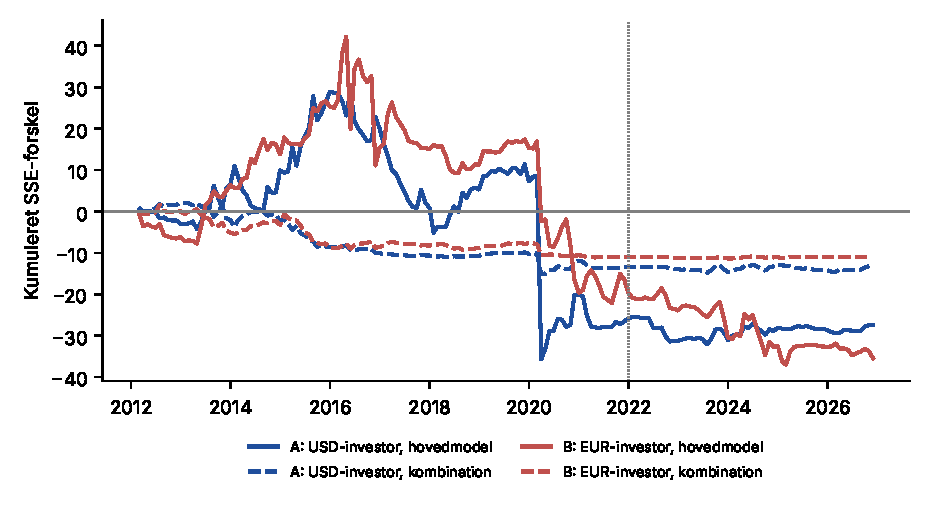
\includegraphics[width=0.86\textwidth]{resultater/fig_oos.pdf}
\caption{Kumuleret forskel i kvadratfejl: historisk gennemsnit minus model. Stigende kurve betyder, at modellen klarer sig bedre. Lodret linje: start på holdout-perioden.}
\label{fig:oos}
\end{figure}

\subsection{På tværs af lande}
Selv om markedet som helhed ikke kan times, kan forskellene mellem landene muligvis forudsiges. Tabel \ref{tab:tv} viser afkastet af strategier, der rangerer alle 12 lande hver måned. En strategi, der køber de fire lande med højest styringsrente og sælger de fire med lavest, har givet 5,3\,\% om året ($t=2{,}35$), og kompositsignalet 6,2\,\% ($t=2{,}55$). Momentum og value har ikke givet noget alene.

\begin{table}[h!]
\centering
\begin{threeparttable}
\caption{Landeallokering: afkast af strategier baseret på signaler på tværs af lande (alle 12 lande)}
\label{tab:tv}
\small
\begin{tabular}{lrrrrrr}
\toprule
 & \multicolumn{3}{c}{Long--short (top 4 -- bund 4)} & \multicolumn{3}{c}{Top 4 -- ligevægtet (aktivt afkast)} \\
\cmidrule(lr){2-4}\cmidrule(lr){5-7}
Signal & Afkast p.a. & $t$ & Sharpe & Afkast p.a. & $t$ & IR \\
\midrule
Carry & $5{,}29$\,\% & $(2{,}35)$ & $0{,}50$ & $3{,}89$\,\% & $(2{,}99)$ & $0{,}64$ \\
Momentum (12--1) & $-1{,}15$\,\% & $(-0{,}44)$ & $-0{,}10$ & $-0{,}13$\,\% & $(-0{,}09)$ & $-0{,}02$ \\
Value (REER) & $0{,}76$\,\% & $(0{,}34)$ & $0{,}07$ & $0{,}30$\,\% & $(0{,}24)$ & $0{,}05$ \\
Komposit & $6{,}17$\,\% & $(2{,}55)$ & $0{,}57$ & $3{,}78$\,\% & $(2{,}79)$ & $0{,}62$ \\
\bottomrule
\end{tabular}

\begin{tablenotes}\footnotesize
\item \emph{Note:} Månedlig rangering af alle 12 lande efter signal; uafdækket afkast for en dollarinvestor næste måned. Long--short: ligevægtet top 4 minus bund 4. Aktivt afkast: top 4 minus ligevægtet gennemsnit af alle lande. Komposit: gennemsnit af standardiserede signaler. 2003--2026 ($N=285$ for carry og komposit). Newey-West $t$-værdier i parentes.
\end{tablenotes}
\end{threeparttable}
\end{table}

Tabel \ref{tab:tv} har dog et problem: den lader strategien vælge Kina og Indien i hele perioden, selv om de først kom med i EMLC i 2020 og 2024. Tabel \ref{tab:bm} retter det og besvarer det kontrafaktiske spørgsmål: hvad ville investoren have fået, hvis hun \emph{ikke} havde fulgt strategien? Her må strategien kun vælge blandt de lande, der havde en positiv vægt i EMLC på tidspunktet, og den sammenlignes med at holde de samme lande med EMLC's vægte, som er det naturlige alternativ for en investor med EMLC som benchmark.

\begin{table}[h!]
\centering
\begin{threeparttable}
\caption{Strategi mod kontrafaktisk benchmark: investerbare lande}
\label{tab:bm}
\small
\setlength{\tabcolsep}{5pt}
\begin{tabular}{lrrrrrr}
\toprule
 & \multicolumn{3}{c}{A: USD-investor} & \multicolumn{3}{c}{B: EUR-investor} \\
\cmidrule(lr){2-4}\cmidrule(lr){5-7}
 & Afkast p.a. & Vol. p.a. & Sharpe & Afkast p.a. & Vol. p.a. & Sharpe \\
\midrule
\multicolumn{7}{l}{\textit{Carry-strategi}} \\
\quad Strategi: top 4, ligevægtet & $6{,}72$\,\% & $16{,}68$\,\% & $0{,}40$ & $7{,}21$\,\% & $13{,}80$\,\% & $0{,}52$ \\
\quad Benchmark: EMLC-vægtet & $4{,}33$\,\% & $12{,}97$\,\% & $0{,}33$ & $4{,}82$\,\% & $9{,}94$\,\% & $0{,}49$ \\
\quad Benchmark: ligevægtet & $4{,}44$\,\% & $13{,}07$\,\% & $0{,}34$ & $4{,}93$\,\% & $9{,}88$\,\% & $0{,}50$ \\
\quad Merafkast mod EMLC-vægtet & $2{,}39^{*}$\,\% & $(1{,}67)$ & IR $0{,}40$ & $2{,}39^{*}$\,\% & $(1{,}67)$ & IR $0{,}40$ \\
\quad Merafkast mod ligevægtet & $2{,}29$\,\% & $(1{,}61)$ & IR $0{,}38$ & $2{,}29$\,\% & $(1{,}61)$ & IR $0{,}38$ \\
\midrule
\multicolumn{7}{l}{\textit{Komposit-strategi}} \\
\quad Strategi: top 4, ligevægtet & $7{,}50$\,\% & $15{,}33$\,\% & $0{,}49$ & $8{,}24$\,\% & $12{,}59$\,\% & $0{,}65$ \\
\quad Benchmark: EMLC-vægtet & $4{,}26$\,\% & $12{,}84$\,\% & $0{,}33$ & $5{,}00$\,\% & $9{,}89$\,\% & $0{,}51$ \\
\quad Benchmark: ligevægtet & $4{,}42$\,\% & $12{,}95$\,\% & $0{,}34$ & $5{,}16$\,\% & $9{,}84$\,\% & $0{,}52$ \\
\quad Merafkast mod EMLC-vægtet & $3{,}25^{**}$\,\% & $(2{,}39)$ & IR $0{,}60$ & $3{,}25^{**}$\,\% & $(2{,}39)$ & IR $0{,}60$ \\
\quad Merafkast mod ligevægtet & $3{,}09^{**}$\,\% & $(2{,}33)$ & IR $0{,}57$ & $3{,}09^{**}$\,\% & $(2{,}33)$ & IR $0{,}57$ \\
\bottomrule
\end{tabular}

\begin{tablenotes}\footnotesize
\item \emph{Note:} Hver måned vælges blandt de lande, der har positiv vægt i EMLC på tidspunktet. Strategi: de fire lande med højest signal, ligevægtet. EMLC-vægtet benchmark: de samme lande vægtet med EMLC's senest kendte valutavægte. Ligevægtet benchmark: de samme lande, lige vægte. Uafdækket afkast næste måned. Carry: 2005--2026 ($N=255$), komposit: 2004--2026 ($N=262$). Merafkastet er det samme for de to investorer, fordi omregningen fra dollar til euro påvirker strategi og benchmark ens. Newey-West $t$-værdier i parentes, IR: informationsratio.
\end{tablenotes}
\end{threeparttable}
\end{table}

Med det investerbare univers har en dollarinvestor, der fulgte kompositstrategien, fået 7,5\,\% om året mod 4,3\,\% ved at holde EMLC-porteføljen. Merafkastet på 3,3 procentpoint er signifikant ($t=2{,}39$) med en informationsratio på 0,60, men strategien har også haft en højere volatilitet (15,3 mod 12,8\,\%). Målt ved Sharpe-ratioen er forbedringen derfor mindre: fra 0,33 til 0,49. For euroinvestoren er niveauerne højere (8,2 mod 5,0\,\% om året), men merafkastet er det samme. Carry alene giver et merafkast på 2,4 procentpoint ($t=1{,}67$), som kun er signifikant på 10\,\%-niveau. Det tidligere resultat for carry var altså delvist drevet af lande, der ikke var investerbare i fonden. H7 understøttes derfor kun delvist. Resultatet er i tråd med \citet{lustig2011} og \citet{asness2013}, men der er set bort fra handelsomkostninger, og afkastet har været større efter 2022 end før.

\subsection{Afdækningsbeslutningen for euroinvestoren}
For en euroinvestor er det centrale spørgsmål ikke kun, om afkastet kan forudsiges, men om valutaen skal afdækkes. Hovedmodellens prognose for euroinvestorens valutaoverskudsafkast ($r^B-r^D$) har et negativt $R^2_{OOS}$ ($-1{,}0$\,\%), men Clark-West-testen er signifikant på 10\,\%-niveau ($p=0{,}05$). Tabel \ref{tab:afd} viser, at afdækningsreglen har hævet Sharpe-ratioen fra 0,36 for en altid uafdækket investor og 0,35 for en altid afdækket investor til 0,41. Reglen har holdt valutaen uafdækket i 66\,\% af månederne. For dollarinvestoren giver reglen ingen gevinst. Her er det mest bemærkelsesværdige, at en altid afdækket dollarinvestor har haft en langt højere Sharpe-ratio (0,50) end en uafdækket (0,18). Valutarisikoen er altså ikke blevet betalt for en dollarinvestor i perioden. H8 understøttes, men forskellen i Sharpe-ratio er ikke testet formelt og bør ses som en indikation.

\begin{table}[h!]
\centering
\begin{threeparttable}
\caption{Afdækningsstrategier uden for stikprøven, 2012--2026}
\label{tab:afd}
\small
\begin{tabular}{lrrrrrr}
\toprule
 & \multicolumn{3}{c}{EUR-investor} & \multicolumn{3}{c}{USD-investor} \\
\cmidrule(lr){2-4}\cmidrule(lr){5-7}
Strategi & Afkast p.a. & Vol. p.a. & Sharpe & Afkast p.a. & Vol. p.a. & Sharpe \\
\midrule
Altid uafdækket & $3{,}37$\,\% & $9{,}44$\,\% & $0{,}36$ & $2{,}15$\,\% & $11{,}86$\,\% & $0{,}18$ \\
Altid afdækket & $1{,}76$\,\% & $5{,}02$\,\% & $0{,}35$ & $2{,}54$\,\% & $5{,}04$\,\% & $0{,}50$ \\
Dynamisk afdækning & $3{,}56$\,\% & $8{,}60$\,\% & $0{,}41$ & $2{,}18$\,\% & $9{,}84$\,\% & $0{,}22$ \\
\bottomrule
\end{tabular}

\begin{tablenotes}\footnotesize
\item \emph{Note:} Vægtet aggregat. Dynamisk afdækning: uafdækket, når hovedmodellen forudsiger positivt valutaoverskudsafkast, ellers afdækket. Afdækning via styringsrenteforskellen. $N=178$.
\end{tablenotes}
\end{threeparttable}
\end{table}

\begin{figure}[h!]
\centering
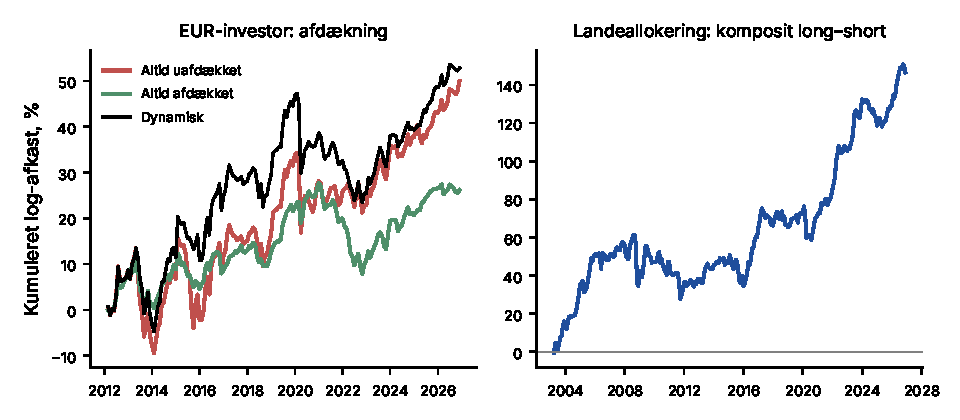
\includegraphics[width=0.9\textwidth]{resultater/fig_strategier.pdf}
\caption{Kumuleret afkast af afdækningsstrategier for euroinvestoren (venstre) og af kompositstrategien på tværs af lande (højre)}
\label{fig:strat}
\end{figure}

\subsection{Robusthed: EMLC-fonden}
Som robusthed er prognoserne gentaget på selve EMLC-fonden for 2015--2026 ($N=136$) i tabel \ref{tab:progemlc}. Resultaterne er de samme: ingen model forudsiger fondens afkast bedre end gennemsnittet, hverken for en dollar- eller en euroinvestor.

\begin{table}[h!]
\centering
\begin{threeparttable}
\caption{Forudsigelse af EMLC-fondens overskudsafkast uden for stikprøven}
\label{tab:progemlc}
\footnotesize
\setlength{\tabcolsep}{4pt}
\begin{tabular}{lrrrrrrrr}
\toprule
 & \multicolumn{4}{c}{EMLC, USD-investor} & \multicolumn{4}{c}{EMLC, EUR-investor} \\
\cmidrule(lr){2-5}\cmidrule(lr){6-9}
Model & $R^2_{OOS}$ & CW $p$ & Hit & $\Delta$CER & $R^2_{OOS}$ & CW $p$ & Hit & $\Delta$CER \\
\midrule
Carry & $-3{,}21$ & $0{,}85$ & $44$ & $-0{,}05$ & $-4{,}80$ & $0{,}61$ & $46$ & $1{,}55$ \\
Dollar-momentum & $-0{,}72$ & $0{,}73$ & $44$ & $-0{,}88$ & $-0{,}53$ & $0{,}46$ & $51$ & $1{,}03$ \\
Valuta-momentum & $-0{,}10$ & $0{,}86$ & $42$ & $0{,}00$ & $0{,}00$ & -- & $54$ & $0{,}00$ \\
Value (REER) & $-0{,}29$ & $0{,}56$ & $48$ & $-0{,}76$ & $-1{,}71$ & $0{,}83$ & $50$ & $-1{,}37$ \\
VIX & $-3{,}75$ & $0{,}79$ & $48$ & $-1{,}65$ & $-4{,}81$ & $0{,}80$ & $53$ & $-0{,}31$ \\
\midrule
Hovedmodel (carry, dollar-mom., VIX) & $-7{,}42$ & $0{,}95$ & $41$ & $-3{,}96$ & $-11{,}66$ & $0{,}65$ & $50$ & $0{,}30$ \\
Kombination (gns. af univariate) & $-1{,}19$ & $0{,}94$ & $40$ & $-1{,}47$ & $-1{,}40$ & $0{,}89$ & $49$ & $-1{,}98$ \\
\bottomrule
\end{tabular}

\begin{tablenotes}\footnotesize
\item \emph{Note:} Som tabel \ref{tab:prog}, men for EMLC-fonden, august 2015 -- november 2026. Prædiktorerne er de samme som for aggregatet.
\end{tablenotes}
\end{threeparttable}
\end{table}

% ---------------------------------------------------------------- diskussion
\section{Diskussion}

Den vigtigste pointe for en europæisk investor er, at dollarrisikoen i EM-obligationer i lokalvaluta afhænger af valutaafdækningen. En uafdækket euroinvestor har næsten ingen dollarrisiko, fordi euroen og EM-valutaerne bevæger sig i samme retning over for dollaren. En euroinvestor i en dollarafdækket andelsklasse har derimod den fulde dollarrisiko. For en dansk investor, hvor kronen er bundet til euroen, gælder det samme. Påstanden i version 1 om, at EM-obligationer er en position på en svagere dollar, gælder altså for en dollarinvestor og for en euroinvestor i en dollarafdækket andelsklasse, men ikke for en uafdækket euroinvestor.

Landesammensætningen betyder dog meget. For en euroinvestor er det de centraleuropæiske lande og Brasilien, der bærer dollarrisikoen, mens de asiatiske lande med styrede valutaer fungerer som en dollarposition. Det er et argument mod at antage, at en regional diversificering automatisk mindsker risikoen: Polen, Tjekkiet og Ungarn ligner euroen i normale måneder, men ikke i de måneder, hvor dollaren stiger kraftigt.

Prognosedelen bekræfter resultatet fra version 1: markedet som helhed kan ikke times med simple variable. Den eneste evidens for forudsigelighed findes på tværs af lande, hvor et kombineret signal har givet et merafkast i forhold til EMLC-porteføljen, og i afdækningsbeslutningen for euroinvestoren. Begge resultater er dog moderate, og de bør bekræftes på nye data, før der lægges vægt på dem.

Analysen har en række begrænsninger. \emph{For det første} bygger obligationsafkastene på én generisk 10-årig obligation pr.\ land og ikke på en indekskurv, og renterne kommer fra investing.com og OECD. Valideringen mod EMLC viser dog, at fejlen er lille. \emph{For det andet} er afdækningen beregnet med styringsrenter og ikke med terminskurser, så afvigelser fra dækket renteparitet \citep{du2018} er ikke med. Det betyder, at afdækningsomkostningen for en euroinvestor sandsynligvis er undervurderet. \emph{For det tredje} dækker de 12 lande kun 68--83\,\% af EMLC, og de resterende lande (bl.a.\ Rumænien, Peru, Chile og Tyrkiet) kan have en anden dollarfølsomhed. Det kan forklare, at aggregatets dollarbeta ($-1{,}35$ i perioden for EMLC) er en anelse større end fondens ($-1{,}26$). \emph{For det fjerde} indgår implicit valutavolatilitet, udenlandsk ejerandel og bytteforhold ikke som prædiktorer, fordi data enten kræver Bloomberg eller ikke var klar. \emph{Endelig} er der testet flere modeller og signaler, hvilket øger risikoen for, at et enkelt signifikant resultat skyldes tilfældigheder.

% ---------------------------------------------------------------- konklusion
\section{Konklusion}

Denne version har undersøgt, hvor dollarfølsomme EM-obligationer i lokalvaluta er i de enkelte lande, hvordan følsomheden afhænger af investorens valuta og afdækning, og om afkastet kan forudsiges.

Analysen viser, at dollarfølsomheden for en dollarinvestor er negativ i 11 af 12 lande og varierer fra $-2{,}0$ i Ungarn til $-0{,}1$ i Kina. Valutaen står for 76\,\% af følsomheden, og obligationsdelen er størst i lande med mange udenlandske investorer. For en uafdækket euroinvestor er dollarbetaen kun $-0{,}19$ og ikke signifikant, mens en euroinvestor i en dollarafdækket andelsklasse har den samme dollarbeta som en dollarinvestor ($-1{,}33$). Afkastet på markedet som helhed kan ikke forudsiges bedre end med det historiske gennemsnit, hverken for en dollar- eller en euroinvestor. Derimod har en strategi, der vælger de fire EMLC-lande med det stærkeste kombinerede signal, givet 3,3 procentpoint mere om året end EMLC-porteføljen, og en simpel afdækningsregel har hævet euroinvestorens Sharpe-ratio fra 0,36 til 0,41.

Samlet set viser analysen, at spørgsmålet ``hvor dollarfølsomme er EM-obligationer i lokalvaluta?'' ikke har ét svar. Svaret afhænger af, hvilke lande man ejer, hvilken valuta man måler i, og hvordan man afdækker.

% ---------------------------------------------------------------- litteratur
\begin{thebibliography}{99}\small
\setlength{\itemsep}{0.15em}
\bibitem[Asness et al.(2013)]{asness2013} Asness, C., Moskowitz, T. og Pedersen, L. (2013). Value and Momentum Everywhere. \emph{Journal of Finance}, 68(3), 929--985.
\bibitem[Avdjiev et al.(2019)]{avdjiev2019} Avdjiev, S., Du, W., Koch, C. og Shin, H. S. (2019). The Dollar, Bank Leverage, and Deviations from Covered Interest Parity. \emph{American Economic Review: Insights}, 1(2), 193--208.
\bibitem[Campbell og Thompson(2008)]{campbell2008} Campbell, J. og Thompson, S. (2008). Predicting Excess Stock Returns Out of Sample: Can Anything Beat the Historical Average? \emph{Review of Financial Studies}, 21(4), 1509--1531.
\bibitem[Clark og West(2007)]{clark2007} Clark, T. og West, K. (2007). Approximately Normal Tests for Equal Predictive Accuracy in Nested Models. \emph{Journal of Econometrics}, 138(1), 291--311.
\bibitem[Du et al.(2018)]{du2018} Du, W., Tepper, A. og Verdelhan, A. (2018). Deviations from Covered Interest Rate Parity. \emph{Journal of Finance}, 73(3), 915--957.
\bibitem[Hofmann et al.(2020)]{hofmann2020} Hofmann, B., Shim, I. og Shin, H. S. (2020). Bond Risk Premia and the Exchange Rate. \emph{Journal of Money, Credit and Banking}, 52(S2), 497--520.
\bibitem[Lustig og Verdelhan(2007)]{lustig2007} Lustig, H. og Verdelhan, A. (2007). The Cross Section of Foreign Currency Risk Premia and Consumption Growth Risk. \emph{American Economic Review}, 97(1), 89--117.
\bibitem[Lustig et al.(2011)]{lustig2011} Lustig, H., Roussanov, N. og Verdelhan, A. (2011). Common Risk Factors in Currency Markets. \emph{Review of Financial Studies}, 24(11), 3731--3777.
\bibitem[Menkhoff et al.(2012)]{menkhoff2012} Menkhoff, L., Sarno, L., Schmeling, M. og Schrimpf, A. (2012). Currency Momentum Strategies. \emph{Journal of Financial Economics}, 106(3), 660--684.
\bibitem[Newey og West(1987)]{newey1987} Newey, W. og West, K. (1987). A Simple, Positive Semi-Definite, Heteroskedasticity and Autocorrelation Consistent Covariance Matrix. \emph{Econometrica}, 55(3), 703--708.
\bibitem[Rapach et al.(2010)]{rapach2010} Rapach, D., Strauss, J. og Zhou, G. (2010). Out-of-Sample Equity Premium Prediction: Combination Forecasts and Links to the Real Economy. \emph{Review of Financial Studies}, 23(2), 821--862.
\bibitem[Verdelhan(2018)]{verdelhan2018} Verdelhan, A. (2018). The Share of Systematic Variation in Bilateral Exchange Rates. \emph{Journal of Finance}, 73(1), 375--418.
\bibitem[Welch og Goyal(2008)]{welch2008} Welch, I. og Goyal, A. (2008). A Comprehensive Look at the Empirical Performance of Equity Premium Prediction. \emph{Review of Financial Studies}, 21(4), 1455--1508.
\end{thebibliography}

\end{document}
